\section{El Proceso De Inicio}\label{sec:el proceso de inicio}

	%The system BIOS is what starts the computer running when you turn it on.
	%The following are the steps that a typical boot sequence involves. Of
	%course this will vary by the manufacturer of your hardware, BIOS, etc., and
	%especially by what peripherals you have in the PC. Here is what generally
	%happens when you turn on your system power:

	\begin{enumerate}
		\item[1]El sistema BIOS es lo que inicia la computadora cuando la
			encendemos.  Los siguientes pasos son los pasos que involucra la
			secuencia de booteo típico.  Por supuesto esto depende del
			fabricante de la hardware, BIOS, etc., y especialmente por los
			perífericos de la PC. Esto es lo que pasa por lo general cuando
			encendemos la energía de la computadora.

	%The internal power supply turns on and initializes. The power supply takes
	%some time until it can generate reliable power for the rest of the
	%computer, and having it turn on prematurely could potentially lead to
	%damage. Therefore, the chipset will generate a reset signal to the
	%processor (the same as if you held the reset button down for a while on
	%your case) until it receives the Power Good signal from the power supply.
	
		\item[2] La fuente de alimentación interna se enciende y se inicializa.
			La fuente de alimentación necesita algún tiempo para generar
			energía seguro para el resto de la computadora, y enciendola antes
			de tiempo potencialmente puede causar daños. Por lo tanto el
			chipset va a enviar una señal de reseteo al procesador (es lo mismo
			que como si uno fuera apretando el botón de RESET) hasta que recibe
			el ``Power Good'' señal de la fuente de alimentación.

	%When the reset button is released, the processor will be ready to start
	%executing. When the processor first starts up, it is suffering from
	%amnesia; there is nothing at all in the memory to execute.  Of course
	%processor makers know this will happen, so they pre-program the processor
	%to always look at the same place in the system BIOS ROM for the start of
	%the BIOS boot program. This is normally location FFFF0h, right at the end
	%of the system memory. They put it there so that the size of the ROM can be
	%changed without creating compatibility problems. Since there are only 16
	%bytes left from there to the end of conventional memory, this location just
	%contains a "jump" instruction telling the processor where to go to find the
	%real BIOS startup program.  
	
		\item[3] Cuando el botón de resteo es liberado, el procesador va a
			estar listo para ejecutar acciones.  Al inidcio el procesador no
			trabaja nada; no hay nada en la memoría para ser procesado.  Por lo
			tanto se carga instrucciones de la BIOS\ref{sec:conceptobios}
			ROM\ref{sec:conceptorom}, normalmente en la posición de la memoría
			FFFF0h, los últimos de 16 bits de la memoría, donde está guardada
			la posición del programa del BIOS booteo o bien POST(Auto
			diagnóstico al encender) para ser procesadas.

	%The BIOS performs the power-on self test (POST). If there are
	%any fatal errors, the boot process stops. POST beep codes can be found in this
	%area of the Troubleshooting Expert.
	
		\item[4] El BIOS realiza el POST(Auto diagnóstico al encebuiltinnder). Si hay une
			error fatal, el proceso de inicio se detiene. Errores son desplegadas
			por una secuencia de pítidos con significados concretos.
	
	%The BIOS looks for the video card. In particular, it looks for the video
	%card's built in BIOS program and runs it.  This BIOS is normally found at
	%location C000h in memory. The system BIOS executes the video card BIOS,
	%which initializes the video card. Most modern cards will display
	%information on the screen about the video card. (This is why on a modern PC
	%you usually see something on the screen about the video card before you see
	%the messages from the system BIOS itself).  The BIOS then looks for other
	%devices' ROMs to see if any of them have BIOSes. Normally, the IDE/ATA hard
	%disk BIOS will be found at C8000h and executed. If any other device BIOSes
	%are found, they are executed as well.  

		\item[5] El BIOS busca la tarjeta de video. En particular, busca el
			Firmware de la tarjeta de video y lo ejecuta. Este firmware
			generalmente se encuentra en la posicion de memoria C000h.  El
			sistema BIOS ejecuta el Firmware de la tarjeta de video, lo cual
			inicializa la tarjeta. La mayoria de las tarjetas de video modernas
			van a desplegar informacion en pantalla acerca de la tarjeta de
			video. (Esta es la razon, por la cual ves mensajes en la pantalla
			al inciar la computadora) El BIOS entonces busca los Firmwares de
			otros dispositivos para ver si estos tienen BIOSes.
				
	%The BIOS displays its
	%startup screen.  
		\item[6] El BIOS muestra la pantalla inicial.
			\begin{figure}[H]
				\centering
					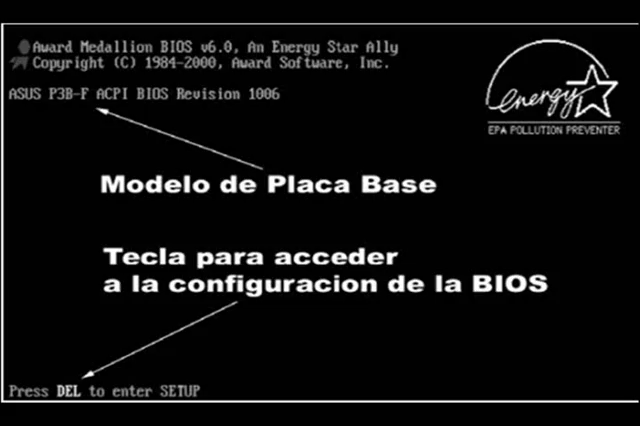
\includegraphics[scale=0.3]{img/Screenshot-Ingresando_al_BIOS_Setup-1.png}
				\caption{El BIOS al encender la computadora.}
			\end{figure}
	
    %The BIOS does more tests on the system, including the memory
	%count-up test which you see on the screen. The BIOS will generally display a
	%text error message on the screen if it encounters an error at this point; these
	%error messages and their explanations can be found in this part of the
	%Troubleshooting Expert.  

	\item[6] El BIOS hace mas pruebas del sistema, incluyendo el conteo de memoria
		RAM. \\
		Generalmente ahora si ocurren errores fatales se los desplegara en la
		pantalla en vez de una notificación auditiva.

	%The BIOS performs a "system inventory" of sorts, doing
	%more tests to determine what sort of hardware is in the system. Modern BIOSes
	%have many automatic settings and will determine memory timing (for example)
	%based on what kind of memory it finds. Many BIOSes can also dynamically set
	%hard drive parameters and access modes, and will determine these at roughly
	%this time. Some will display a message on the screen for each drive they detect
	%and configure this way. The BIOS will also now search for and label logical
	%devices (COM and LPT ports).  

	%If the BIOS supports the Plug and Play standard,
	%it will detect and configure Plug and Play devices at this time and display a
	%message on the screen for each one it finds. See here for more details on how
	%PnP detects devices and assigns resources.  
	\item[7] El BIOS ahora realiza un sistema de inventario de sorteos, haciendo
		más pruebas para determinar el tipo de hardware del sistema.
		BIOSes modernos tienen ajustes automáticos y determinarán la sincronización
		de la memoría (por ejemplo) basado en que tipo de memoría de encuentra.
		Muchos BIOSes tambien pueden determinar {\em automáticamente} parametros
		del disco duro y los modos de acceso, y determinará estos aproximadamente
		en este período.
		Algunas desplegarán un mensaje en la pantalla para cada unidad/dispositivo que
		se detecta y lo configura a esa manera. El BIOS ahora buscará y calificará los
		dispositivos lógicos. \\*
		Si el BIOS soporta el estándar {\emph Plug-and-Play }\cite{plugandplay} este detectará
		y configurará los dispositivos {\emph Plug-and-Play} mientras y mostrará un mensaje
		en pantalla para cada dispositivo registrado.
	
	%The BIOS will display a summary
	%screen about your system's configuration. Checking this page of data can be
	%helpful in diagnosing setup problems, although it can be hard to see because
	%sometimes it flashes on the screen very quickly before scrolling off the top.

	\item[8] El BIOS mostrará un resumen en pantalla de la configuración del sistema.  Revisando
		esta página puede ayudar en diágnosticar problemas con la configuración, a
		pesar de que lo puede resultar díficil porque se despide muy rapidamente. \\
		{\bf Truco:} Apretar la tecla <PAUSE>.

	%The BIOS begins the search for a drive to boot from. Most modern BIOSes contain
	%a setting that controls if the system should first try to boot from the floppy
	%disk (A:) or first try the hard disk (C:). Some BIOSes will even let you boot
	%from your CD-ROM drive or other devices, depending on the boot sequence BIOS
	%setting.
	
	%Having identified its target boot drive, the BIOS looks for boot
	%information to start the operating system boot process. If it is searching a
	%hard disk, it looks for a master boot record at cylinder 0, head 0, sector 1
	%(the first sector on the disk); if it is searching a floppy disk, it looks at
	%the same address on the floppy disk for a volume boot sector.
	
	%If it finds what
	%it is looking for, the BIOS starts the process of booting the operating system,
	%using the information in the boot sector. At this point, the code in the boot
	%sector takes over from the BIOS. The DOS boot process is described in detail
	%here. If the first device that the system tries (floppy, hard disk, etc.) is
	%not found, the BIOS will then try the next device in the boot sequence, and
	%continue until it finds a bootable device.  
	
	%If no boot device at all can be
	%found, the system will normally display an error message and then freeze up the
	%system. What the error message is depends entirely on the BIOS, and can be
	%anything from the rather clear "No boot device available" to the very cryptic
	%"NO ROM BASIC - SYSTEM HALTED". This will also happen if you have a bootable
	%hard disk partition but forget to set it active.  
	
	%This process is called a
	%"cold boot" (since the machine was off, or cold, when it started). A "warm
	%boot" is the same thing except it occurs when the machine is rebooted using
	%{Ctrl}+{Alt}+{Delete} or similar. In this case the POST is skipped and the boot
	%process continues roughly at step 8 above.

	\item[9] La próxima tarea del BIOS consiste en buscar un sistema operativo
		la cual cargará en la memoría. Si la busqueda fue exitosa, el BIOS se despide
		y vemos normalmente la pantalla de carga del sistema operativo.

	\end{enumerate}
	\newpage

